Fixed effects:
                                             Estimate Std. Error         df     t value     Pr(>|t|)    
(Intercept)                                 5.356e-01  9.258e-03  9.796e+02      57.846     < 2e-16 ***
trial_type.effect2                          3.160e-02  1.852e-02  9.796e+02      1.706      0.0883 .  
epoch.effect2                               1.057e-01  1.820e-02  9.768e+02      5.805      8.70e-09 ***
grasp_num                                  -5.348e-03  7.268e-04  9.570e+02     -7.359      4.00e-13 ***
trial_type.effect2:epoch.effect2            8.775e-03  3.641e-02  9.768e+02      0.241      0.8096    
trial_type.effect2:grasp_num               -5.696e-03  1.453e-03  9.570e+02     -3.919      9.53e-05 ***
epoch.effect2:grasp_num                    -2.929e-03  1.428e-03  9.542e+02     -2.051      0.0406 *  
trial_type.effect2:epoch.effect2:grasp_num -3.990e-03  2.857e-03  9.542e+02     -1.397      0.1629    




Linear mixed model fit by REML. t-tests use Satterthwaite's method [
lmerModLmerTest]
Formula: sym_index ~ 1 + trial_type.effect * epoch.effect * grasp_num +  
    (1 | subject_id)
   Data: df
Control: lmerControl(optimizer = "bobyqa", optCtrl = list(maxfun = 2e+05))

REML criterion at convergence: -1195.2

Scaled residuals: 
     Min       1Q   Median       3Q      Max 
-2.98206 -0.68409 -0.01129  0.71463  2.72487 

Random effects:
 Groups     Name        Variance  Std.Dev.
 subject_id (Intercept) 0.0007136 0.02671 
 Residual               0.0278784 0.16697 
Number of obs: 1740, groups:  subject_id, 48

Fixed effects:
                                             Estimate Std. Error         df
(Intercept)                                 5.211e-01  1.324e-02  4.786e+02
trial_type.effect2                          1.235e-01  2.441e-02  1.720e+03
epoch.effect2                               8.133e-02  2.399e-02  1.692e+03
grasp_num                                  -3.048e-03  1.168e-03  1.167e+03
trial_type.effect2:epoch.effect2            1.449e-01  4.801e-02  1.696e+03
trial_type.effect2:grasp_num               -1.534e-02  2.262e-03  1.627e+03
epoch.effect2:grasp_num                     1.395e-03  2.198e-03  1.695e+03
trial_type.effect2:epoch.effect2:grasp_num -1.900e-02  4.397e-03  1.698e+03
                                           t value Pr(>|t|)    
(Intercept)                                 39.362  < 2e-16 ***
trial_type.effect2                           5.061 4.62e-07 ***
epoch.effect2                                3.389 0.000717 ***
grasp_num                                   -2.611 0.009144 ** 
trial_type.effect2:epoch.effect2             3.019 0.002578 ** 
trial_type.effect2:grasp_num                -6.782 1.65e-11 ***
epoch.effect2:grasp_num                      0.635 0.525595    
trial_type.effect2:epoch.effect2:grasp_num  -4.321 1.64e-05 ***
---
Signif. codes:  0 '***' 0.001 '**' 0.01 '*' 0.05 '.' 0.1 ' ' 1

Correlation of Fixed Effects:
            (Intr) trl_.2 epch.2 grsp_n tr_.2:.2 t_.2:_ ep.2:_
trl_typ.ff2 -0.044                                            
epoch.ffct2  0.093 -0.004                                     
grasp_num   -0.884  0.269 -0.102                              
trl_ty.2:.2 -0.005  0.099 -0.019  0.034                       
trl_typ.2:_  0.276 -0.915  0.033 -0.506 -0.104                
epch.ffc2:_ -0.098  0.033 -0.915  0.123  0.254   -0.070       
trl_.2:.2:_  0.033 -0.104  0.254 -0.071 -0.916    0.126 -0.485
 
\textcolor{Blue}{Figure \ref{figure:F_value_exe}} shows the correlation of relative net transitions (F-value) during action execution and number of object displacements within a trial. For EASY trials, Pearson correlation showed the F-value negatively correlated with the number of object displacements ($\rho$=-0.05, p=0.16) which was not significant. For HARD trials, F-values were significantly correlated with number of object displacements ($\rho$=-0.25, p<0.000). These results show that within higher task complexity, subjects' had reduced gaze guidance towards the task-relevant objects in the moment and correlated with sub-optimal behavior in terms of number of object displacements needed to finish the task. We can further conclude that subjects' "indecision" during the action execution epochs was more prevalent in the complex task conditions.

\begin{figure}[h]
    \centering
    \subfloat[]{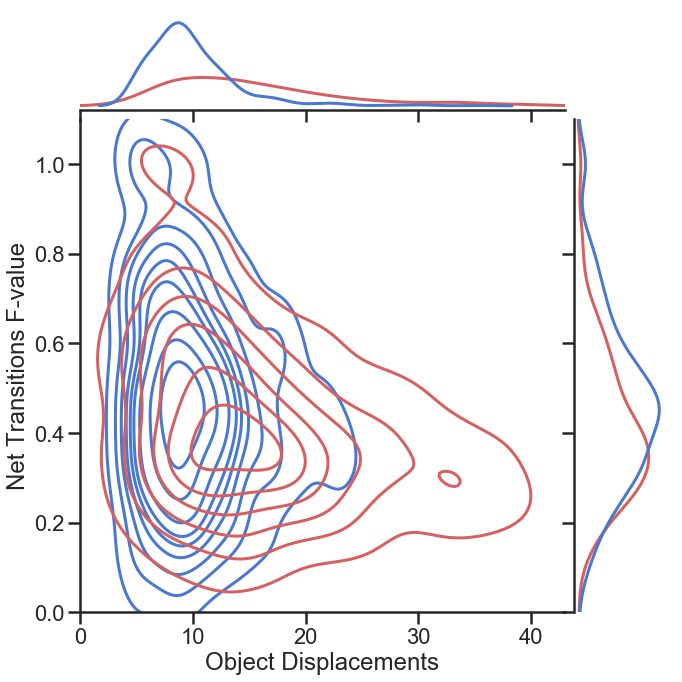
\includegraphics[width=0.3\linewidth]{source/figures/results/gaze_guidance_v_grasps_kde_execution.png}
    \label{figure:g_kde_exe}}
    \subfloat[]{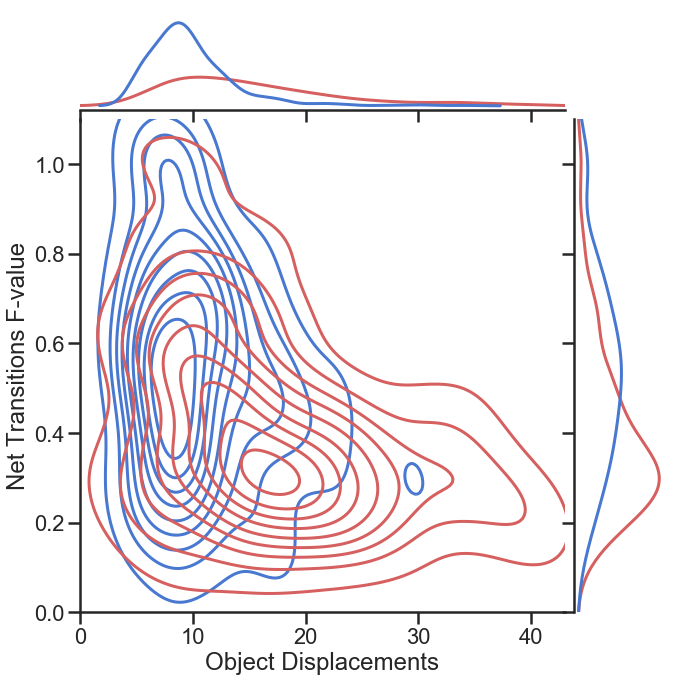
\includegraphics[width=0.3\linewidth]{source/figures/results/gaze_guidance_v_grasps_kde_planning.png}\label{figure:g_kde_plan}}
    \caption[]{Bi-variate kernel density estimate of net-transitions per trial vs. number of object displacement
    Panel \protect\subref{figure:g_kde_exe} shows kde of execution epochs
    Panel \protect\subref{figure:g_kde_plan} shows kde of planning epochs}
     \label{figure:kde}
\end{figure}

\begin{figure}[h]
    \centering
    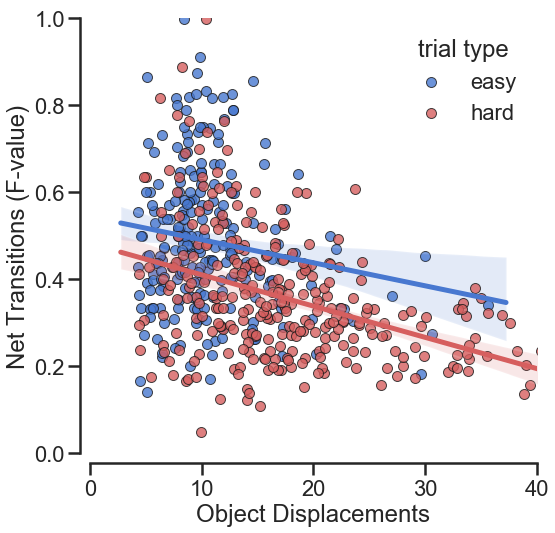
\includegraphics[width=0.3\linewidth]{source/figures/results/gaze_guidance_v_grasps_planning.png}
    \caption[]{Gaze guidance behavior vs. number of object displacements. Figure shows a scatter plot of the relative net transition (F-value) vs. number of object displacements per trial and subject differentiated the two trial types EASY(blue), HARD(red). Each point refers to one trial and it's F value vs. the number of object displacements in that trial. The lines denote the regression fit and the shaded region denotes 95\% confidence interval. F-values for both trial types decrease with increasing number of object displacements. Specifically, higher number of object displacements in a trial is correlated with lower gaze guidance. Pearson correlation $\rho$= -0.15 (p = 0.01) for EASY trials and $\rho$ = -0.38 (p <0.001) for HARD trials\\
    }
    \label{figure:F_value_plan}
\end{figure}